\section{Temporal Verification}
In the temporal verification stage, we will use the path information that we got from 
functional verification stage and augment them with latency information to 
produce the final temporal property probability.

\begin{figure}[h]
    \centering
    % 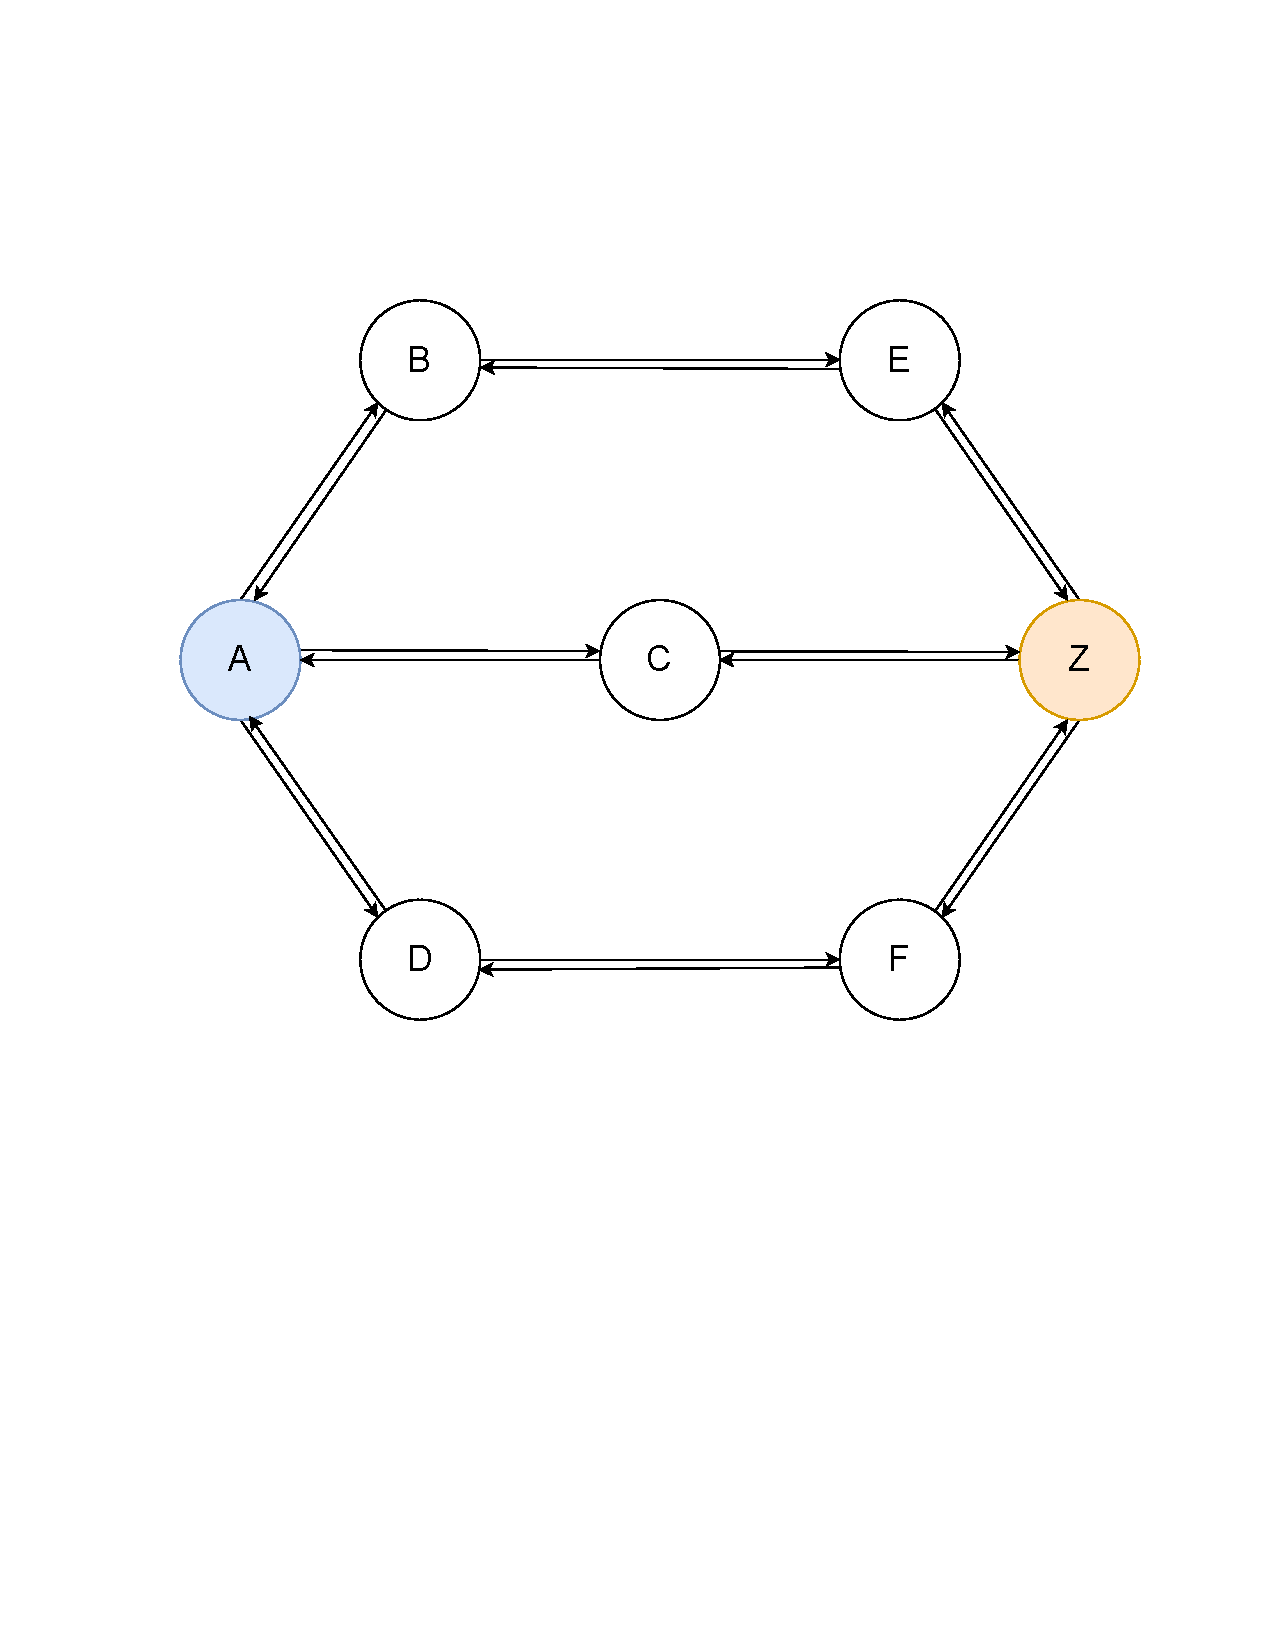
\includegraphics[width=0.4\textwidth, trim=0cm 11cm 0cm 5cm]{ex.pdf}
    \includegraphics[width=\columnwidth]{../tikz/tree}
    % 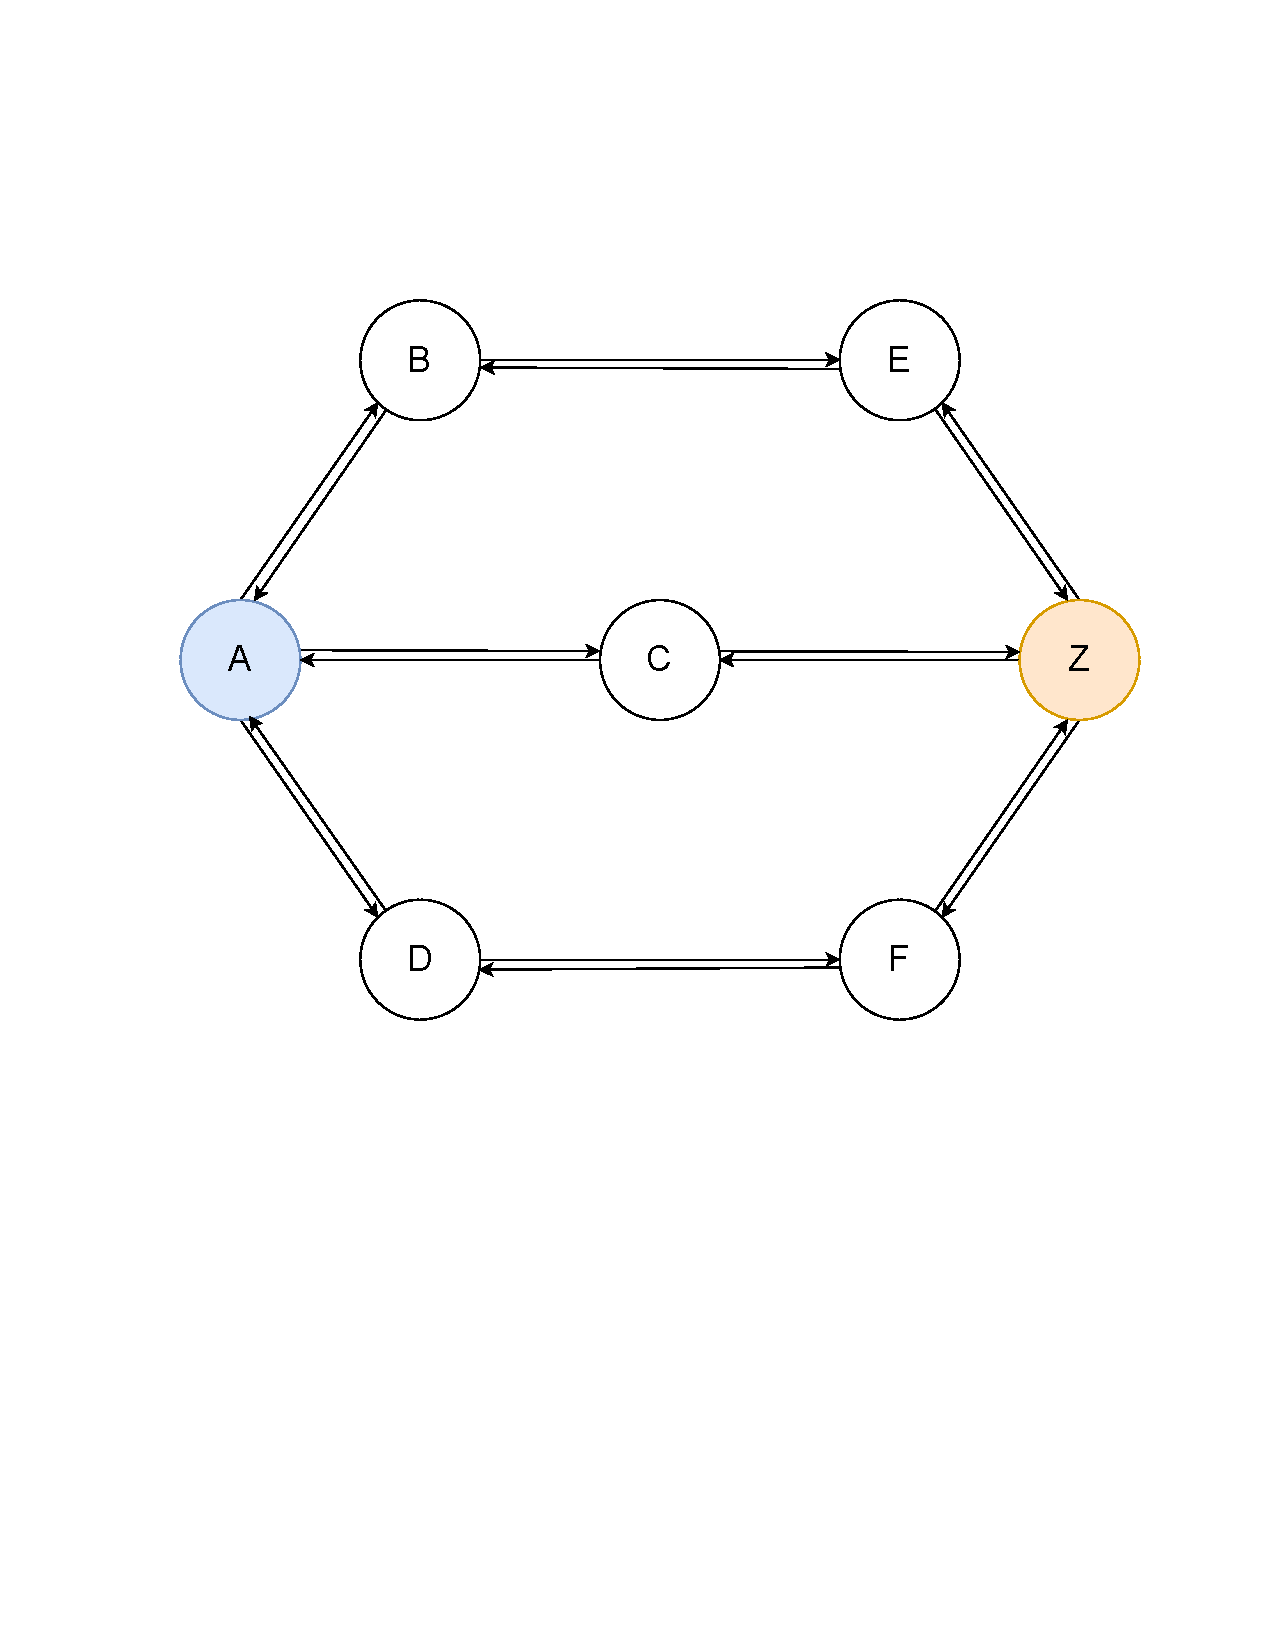
\includegraphics{ex.eps}
    \caption{Subset of Modified Exploration Tree $\mathcal{T}$ for our example topology, 
        $\mathcal{E}_2$ and $\mathcal{E}_3$ will get consolidated}
    \label{fig:tree}
\end{figure}

\subsection{Latency Label}
Similar to link failure $r$, we use edge-labeling technique to represent latency that 
will get introduced by the connectivity between two nodes. 
Our model will model two significant sources of latency: \textbf{link propagation} 
and \textbf{packet queuing in the node}.
We will encode these latencies by equipping the model with two additional labels.

Encoding link propagation latency is fairly straightforward. 
We define a function $l_p: E_t \rightarrow \mathcal{D}$ where $\mathcal{D}$ is a set of 
continuous univariate distribution that has a minimum value of $0$.
This distribution signifies the time it would take for the respective physical link to transmit 
a packet from one end to another.
Because of this, just like $r$, two symmetrical edges will share the same distribution.

To encode queuing latency, we first note that the queuing mechanism in modern switches 
usually resides in the output port. %TODO: Cite PISA?
Since a port in a switch is only connected to one other port, we could effectively 
assign the latency to the connectivity between switches.
To do this, we define another function $l_q: E_t \rightarrow \mathcal{D}$.
This distribution signifies the output queue latency in the source node that is 
going to be forwarded to the destination node.
Unlike $l_p$, two symmetrical edges will have two different distributions since they 
represent two different output queues.

In our running example, we will assume that all edges in the topology will have $l_p$
and $l_q$ of gamma distribution with $\lambda = 1$, except $l_q(EZ)$ which will 
have a lognormal distribution with $\alpha = 1$ and $\theta = 1$.

Given $paths$, $l_p$, and $l_q$, we could then compute $P_t$, the probability of a 
given temporal property being fulfilled.
We will describe our algorithm for computing this probability in the next few 
sections.

\subsection{Weighted Average and Path Convolution}
Since a convergent behavior of the forwarding plane $paths$ might contain more than 
one paths, we will compute the temporal probability of $paths$ by computing the 
weighted average of the temporal probability of each of the individual path.
The specific weight depends on the load-balancing method used.
%We have implemented the weight computation for ECMP load-balancing scheme.

To get the temporal probability of a single path, we will use the latency information 
from $l_p$ and $l_q$ to compute the latency distribution of the whole path.
To do this, we resort to the methods of \textbf{convolution}.
For each edge $e$ in the path, we will get $l_p(e)$ and $l_q(e)$ and convolve them 
all together to get the path latency distribution.

With this path latency distribution, we could get the temporal probability of a 
path by computing the statistical property of said distribution.
In this work, given a path latency distribution $\mathcal{L}$, we define two temporal 
properties:
\begin{itemize}
    \item \textbf{Bounded Reachability}: the probability that a packet will get 
        transmited below $t$ time unit. This will get computed as $cdf(\mathcal{L}, t)$
    \item \textbf{Tail Reachability}: the probability that a packet will get 
        transmited above $t$ time unit. This will get computed as 
        $1 - cdf(\mathcal{L}, t)$
\end{itemize}

In our Fig. \ref{fig:tree} Exploration Tree for example, $\mathcal{E}_2$ has two 
equally probable path, $ABEZ$ and $ADFZ$.
We will first do a chain convolution of all the distributions in $ABEZ$ ($l_p(AB)$, 
$l_q(AB)$, ..., $l_q(EZ)$) and do the same thing for $ADFZ$.
We will then take the $CDF$ of $\mathcal{L}_{ABEZ}$ and $\mathcal{L}_{ADFZ}$ with our 
desired $t$ and average them out to get $P_t$ of $\mathcal{E}_2$. 

In short, given $paths$, $l_p$, and $l_q$, we will do the following:
\begin{enumerate}
    \item Split $paths$ into its individual path
    \item For each path, compute its latency distribution by convolving the latency distribution 
        $l_p$ and $l_q$ of each link
    \item With the resulting path latency distribution, determine the probability of temporal 
        property by computing the statistical property of said distribution
    \item Combine the temporal property of each path by computing the weighted average, based 
        on the load-balancing scheme of the control plane
\end{enumerate}

We do each of these steps to every Equivalence Class in $\mathcal{T}$, and do a sum-product operation 
of $P_f$ and $P_t$ to get the final probability of the property in question.

By introducing the temporal verification algorithm, we're essentially adding additional overhead to the 
exploration algorithm (on top of functional verification) that scales to the size of the Exploration Tree.
In other words, for $\mathcal{T}$ of size $n$, we will need to do temporal verification in each of 
those $n$ Equivalence Class.
We aim to minimize the overhead of temporal verification by introducing some optimization algorithms
later.

\subsection{Numeric Convolution}
However, there is one major problem with a convolution-based technique for computing the latency distribution 
of a given path: not every distribution pair can be convolved analytically.
A closed-form solution of a convolution is usually only available for two distributions of the same type.

In our example, we define $l_q(EZ)$ to be lognormal distribution, which doesn't have a closed form convolution 
solution with the other latency distribution in the network, which is of gamma distribution form.
Therefore, in order to convolve two arbitrary distributions, we need to leverage a numerical convolution 
method.

We leverage an existing numerical convolution algorithm, DIRECT, to fulfill this role.
%TODO: describe DIRECT in one sentence
We choose this method due to their bounded error property: DIRECT guarantee that the computed 
distribution and the correct theoretical distribution has a KL-divergence below a certain bound.
DIRECT has also been implemented in R's popular bayesmeta package.
%TODO: cite and change font?

One subtle detail about DIRECT is while convolution is defined to be a commutative operation, and 
DIRECT also achieves this property, the order of operation matters for the algorithm's runtime 
performance.
In particular, if we had a chain of DIRECT convolutions, the result of a convolution should not be set 
as the second input distribution in the later convolutions to avoid performance penalty.
This is caused by a nested loop from the following two mechanisms:
\begin{itemize}
    \item DIRECT works by computing a list of support values by doing many PDF queries of the second input
        distribution
    \item Computing the PDF of a DIRECT distribution (the returned distribution of a DIRECT 
        algorithm) itself involves iterating over the current support values
\end{itemize}

As an ilustration, if we had 3 random variables $A$, $B$, and  $C$, and we want 
to convolve them all together, it would be faster to compute $direct(direct(A, B), C)$ instead of 
$direct(C, direct(A, B))$.

While this problem is trivial to solve (swap the input parameter if the latter is detected as a 
DIRECT distribution), it does limit the type of optimization that we could have in the chain convolution 
process.

\section{Optimization}
\subsection{Equivalence Class Consolidation}
To minimize the amount of temporal verification overhead, we want to find some symmetry in the 
existing exploration algorithm so that we could reduce the exploration space even further.

In the original NetDice exploration algorithm, multiple network states were merged into an Equivalence 
Class based on its cold edges (edges whose failure won't change the convergent path(s)).
In other words, network states within the same Equivalence Class will have the same convergent path(s).

However, we observe that each of those Equivalence Classes are not \textit{unique}: while network states within 
the same equivalence class shares a convergent path(s), \textbf{multiple equivalence classes could also 
share the exact same convergent path(s)}, as shown in $\mathcal{E}_2$ and $\mathcal{E}_3$ in Fig. \ref{fig:tree}.

Since we define latency distribution to marginalize over all factors other than the path, we could 
effectively \textit{consolidate} these equivalence classes into one big equivalence class and do temporal 
verification once.

We implemented this idea by doing memoization on the temporal probability of a given convergent path(s).
We will only do temporal probability computation once, when we first iterate over an equivalence class that 
has a certain convergent path(s), and we cached the result should another equivalence class with the same 
convergent path(s) emerged.

\subsection{Path Memoization}
After consolidating many equivalence classes that shares the same convergent path(s), we are left with fewer, 
bigger, but unique equivalence classes.
As significant as it is, we could reduce the computation cost further by drawing connections between these 
unique equivalence classes.

In a network with a load-balancing protocol, the convergent state of the data plane might forward a packet 
through multiple possible paths.
In the context of our framework, we say that an equivalence class might have more than one convergent paths.
Nevertheless, we note that two equivalence classes with different convergent paths might not be two 
independent subset.
In other words, \textbf{multiple equivalence classes could share a subset of individual path}.

Since the way we compute convergent path(s) temporal probability is by calculating the weighted average of 
individual path temporal probability, we could reduce the amount of convolution we will need to do by doing further memoization 
on the temporal probability of a given path.
If we were to compute the temporal probability of an equivalence class with previously cached individual 
path, we only need to calculate the weights that corresponds to the load balancing protocol without 
doing any convolution.

In our running example, we could see that in Fig. \ref{fig:tree}, $\mathcal{E}_2$ and $\mathcal{E}_4$ share 
an identical path, $ADFZ$.
We could therefore memoize $cdf(\mathcal{L}_{ADFZ}, t)$ when we explore $\mathcal{E}_2$ and query the 
cached result when we explore $\mathcal{E}_4$.

With this optimization, we will do a chain convolution by the amount of path available in the network between 
the source and destination (which is 3 in the case of our running example in Fig. \ref{fig:ex}: $ACZ$, $ABEF$, 
and $ADFZ$).

\subsection{Convolution Grouping}
Aside from optimizing the \textit{amount} of paths we need to do convolution on, we could also do some 
optimization on the \textit{convolution operation itself}. 

\begin{figure}[h]
    \centering
    % 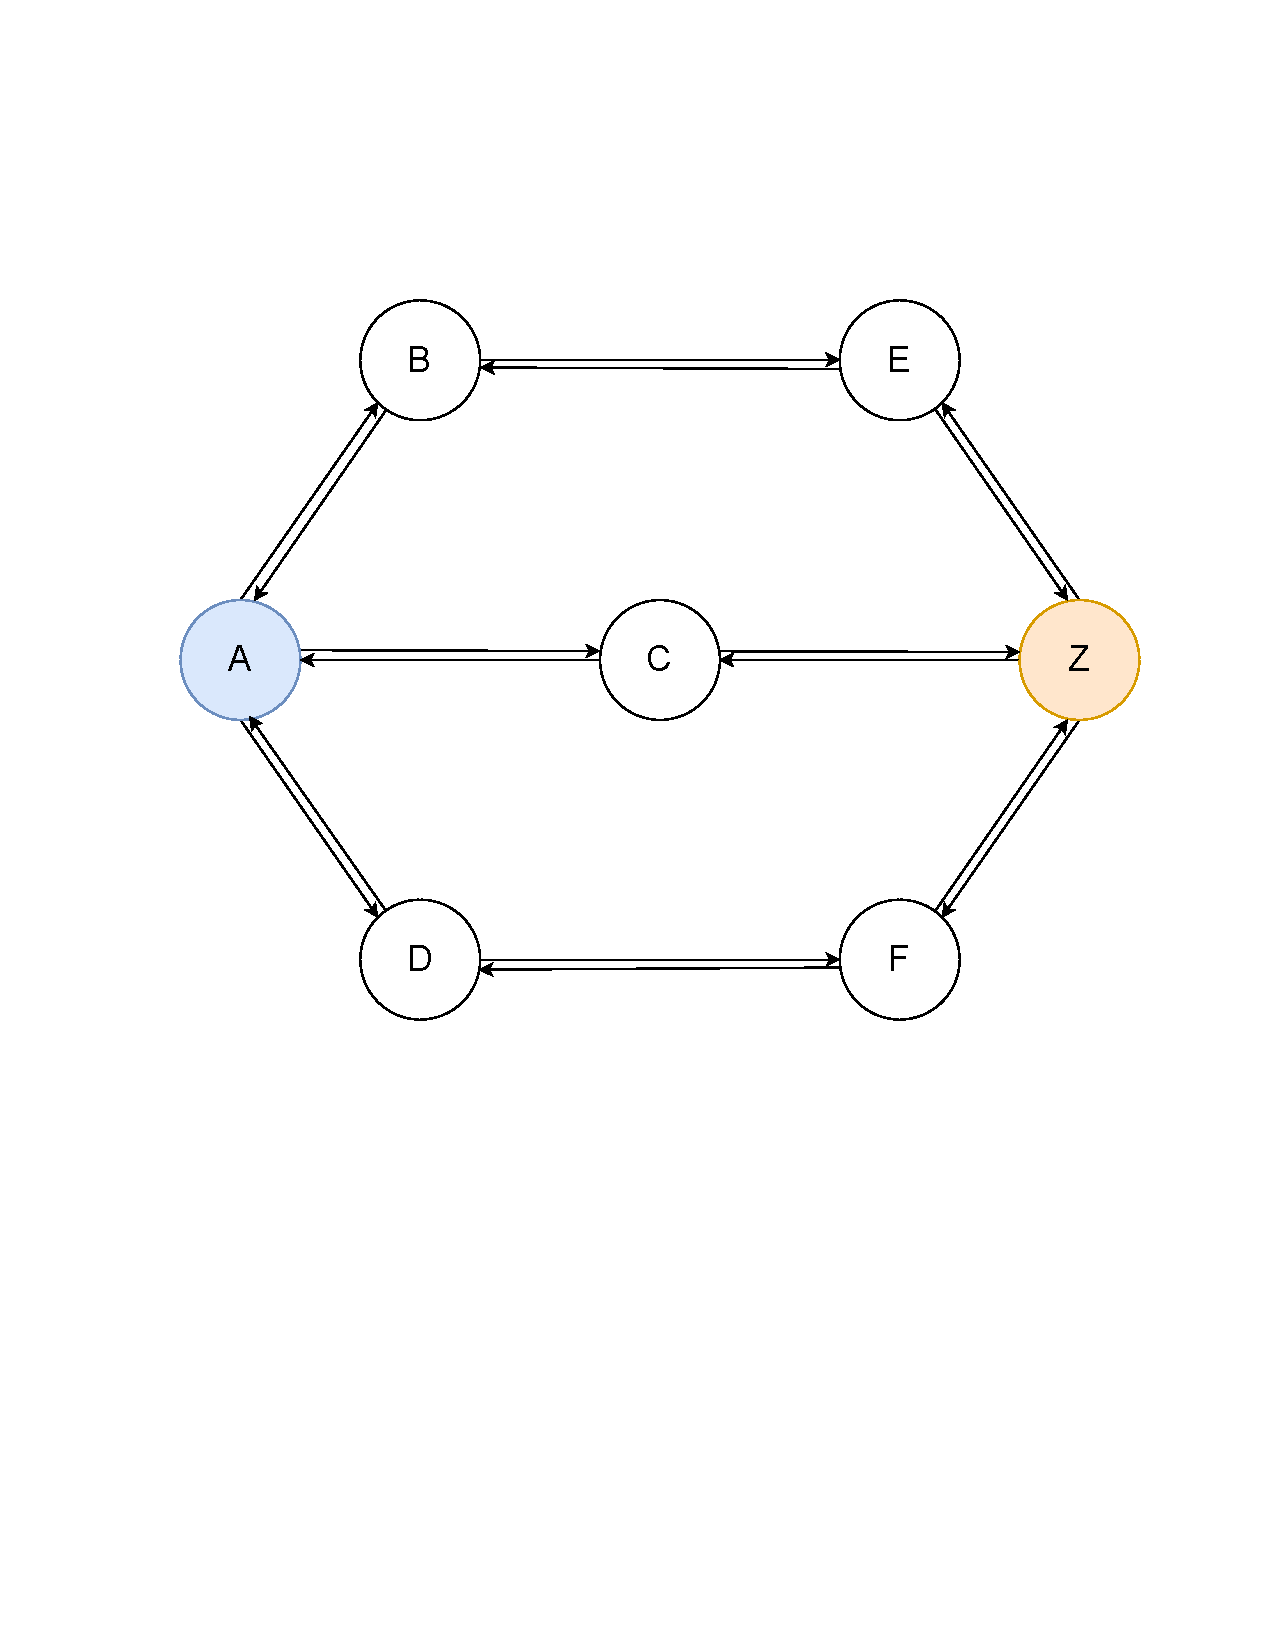
\includegraphics[width=0.4\textwidth, trim=0cm 11cm 0cm 5cm]{ex.pdf}
    \includegraphics[width=\columnwidth]{../tikz/group}
    % 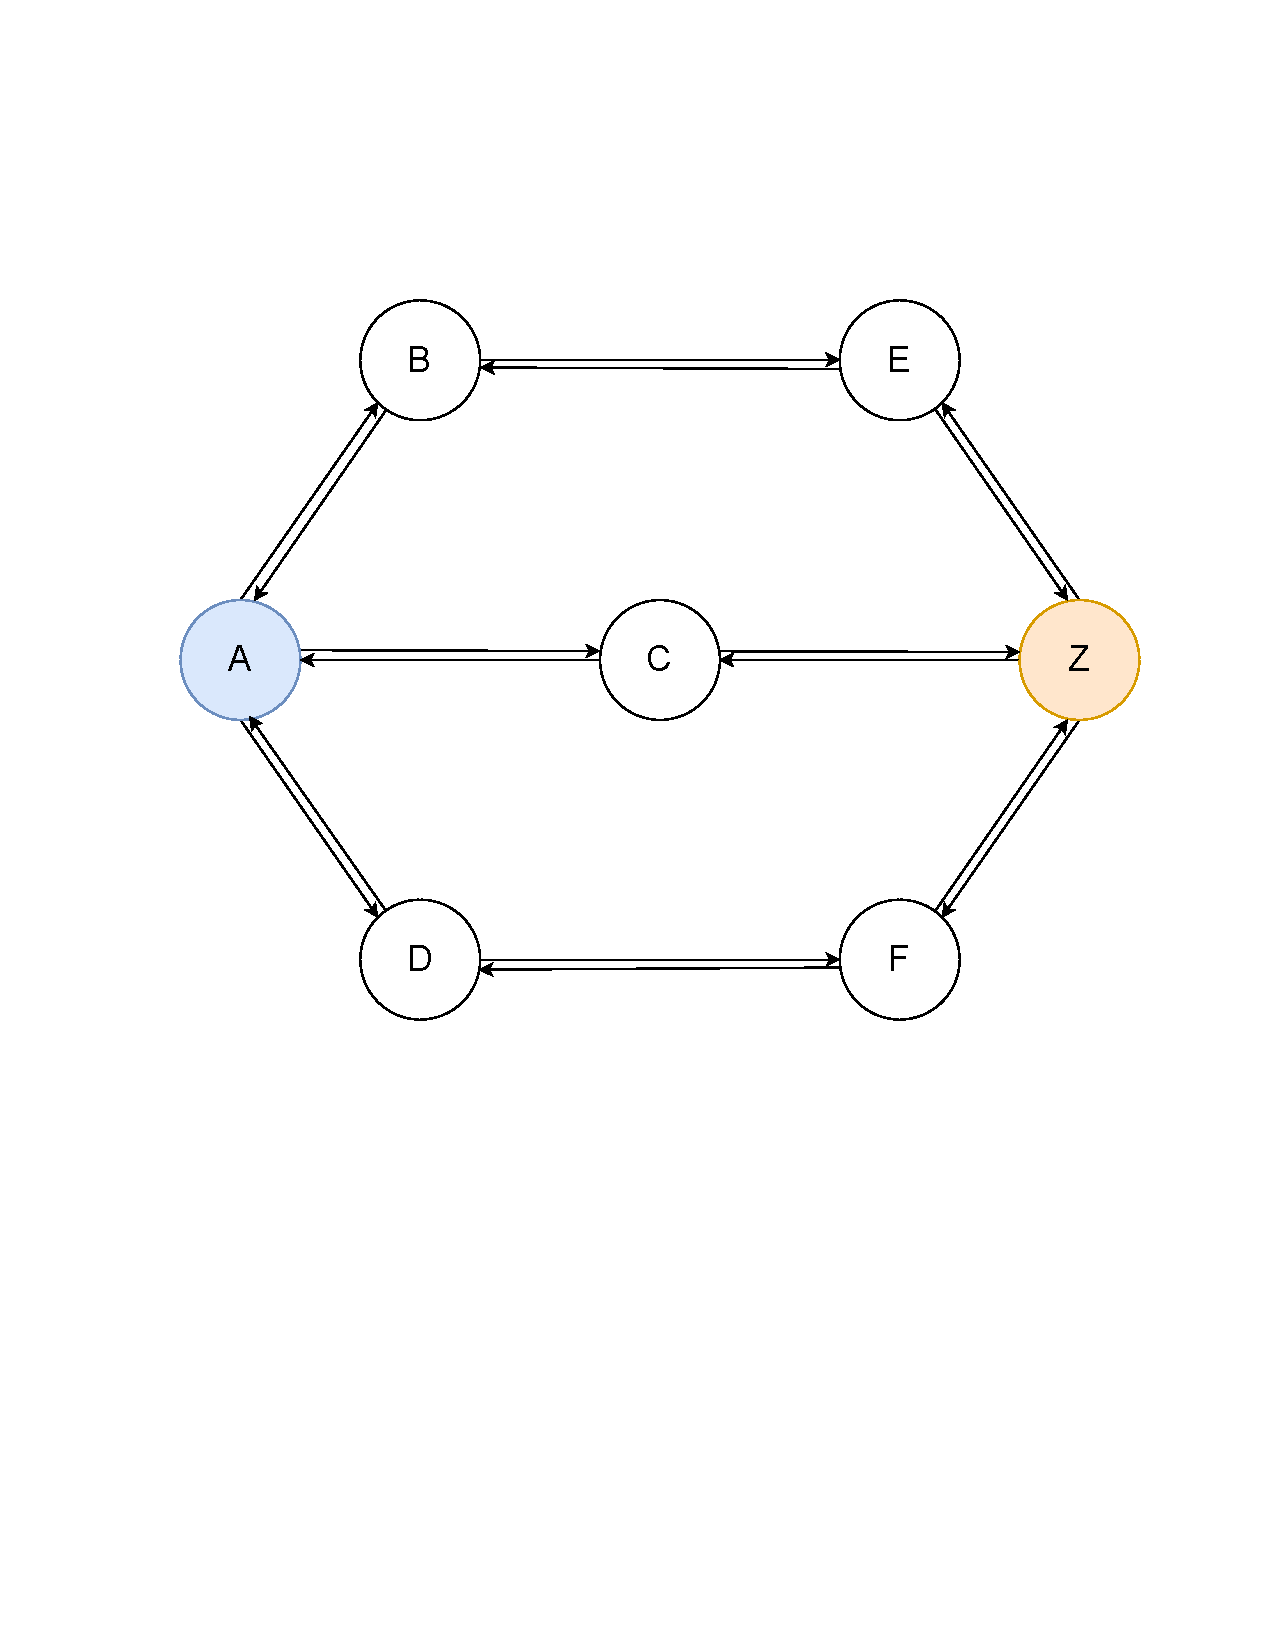
\includegraphics{ex.eps}
    \caption{One example of a convolution tree to get $\mathcal{L}_{ABEZ}$ with optimized grouping,
    we want to start introducing numerical convolution as late as possible}
    \label{fig:grouping}
\end{figure}

While the use of numerical technique to do convolution enabled us to use arbitrary probability distribution 
in our framework, it comes with two noticeable disadvantages.

The first is \textit{error}: numerical method is fundamentally an approximation technique that always 
comes with some error. 
While DIRECT algorithm comes with an error-bound guarantee, it is not zero and could expand if we do 
chain convolution.

The second is \textit{runtime performance}: even with the input ordering constraints we laid out on the 
previous subsection, DIRECT is still generally slower than analytical convolution.
This is expected, since a closed form solution of a convolution tipically boils the operation down into 
a few arithmetic calculation, rather than complex operation like integration.
Due to these factors, we feel the need to \textbf{prioritize analytical convolution} in the calculation of 
path latency distribution.

We did this by \textit{grouping} subsets of the path components with the same probability distribution 
type (e.g. exponential, normal, etc.). 
We then analytically convolve the distribution within that subset and only numerically convolve the 
returned distribution, which will be fewer in quantity, thus enabling smaller error and faster performance.

In our running example, in the chain convolution process to get $\mathcal{L}_{ABEZ}$, we will analytically
convolve $l_p(AB)$, $l_q(AB)$, $l_p(BE)$, $l_q(BE)$, and $l_p(EZ)$ since they are of the same type (gamma) 
and then numerically convolve the resulting distribution with $l_q(EZ)$.
Fig. \ref{fig:grouping} illustrates how the chain convolution process will be broken down.

% \textbf{First}, we do the functional verification with $G_t$ similar to what NetDice 
% \cite{steffen2020probabilistic} have done. 
% In addition, we also collect additional information from each state (e.g. convergent 
% paths) to be used in the temporal verification step. 

% \textbf{Second}, we compute the total path latency distribution from the convergent path(s) in each 
% state with $G_l$.
% This is done by convolving over the latency distribution of each component in the path. 
% Since not all convolutions can be calculated analytically, we implemented a numerical convolution 
% method via mixture distribution, DIRECT \cite{rover2017discrete}, which is able to convolve two 
% distribution with a KL divergence error bound.
% Multiple states can share the same convergent path(s), so \textit{only a fraction of the states need to be 
% explored}.

% \textbf{Third}, we calculate the probability of a given temporal property being true in that state. 
% For example, given a \textit{bounded reachability property} (probability of whether a packet can 
% traverse from a source to destination below some time unit $T$), we can compute its probability by 
% integrating the PDF from $0$ to $T$. 
% We then combine all of the \textit{temporal} and \textit{functional} probability in each state to 
% get the final probability: the probability of \textit{the network} fulfilling a temporal property.

% TODO: intro, reformalize graph formulation, citations
% Does a figure about topology graph and latency graph will be useful?
% Multimedia context on older networked system Klara Nahrstedts
% Graph 